\PassOptionsToPackage{dvipsnames}{xcolor}
\documentclass[tikz]{standalone}
\usepackage[]{amsmath}
\usetikzlibrary{positioning}

    %\path [fill = <++>, draw = <++>, line width = 4] (<++>) circle [radius = 0.3];

\DeclareMathOperator{\col}{col}
\def\vertexcolor{\color{BrickRed}}
\def\edgecolor{\color{ForestGreen}}
\def\v#1{{\vertexcolor#1}}
\def\e#1{{\edgecolor#1}}
\begin{document}
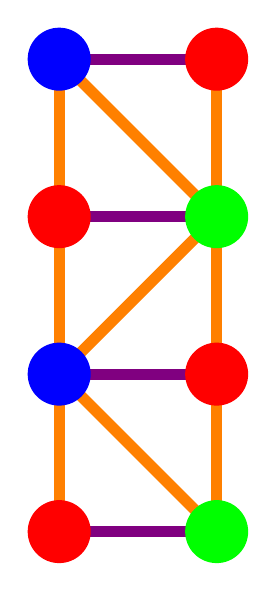
\begin{tikzpicture}
    \draw [violet, line width = 4] (0,0) -- (2,0);
    \draw [violet, line width = 4] (0,2) -- (2,2);
    \draw [violet, line width = 4] (0,4) -- (2,4);
    \draw [violet, line width = 4] (0,6) -- (2,6);

    \draw [orange, line width = 4] (0,0) -- (0,2);
    \draw [orange, line width = 4] (0,2) -- (0,4);
    \draw [orange, line width = 4] (0,4) -- (0,6);

    \draw [orange, line width = 4] (2,0) -- (2,2);
    \draw [orange, line width = 4] (2,2) -- (2,4);
    \draw [orange, line width = 4] (2,4) -- (2,6);

    \draw [orange, line width = 4] (0,2) -- (2,0);
    \draw [orange, line width = 4] (0,2) -- (2,4);
    \draw [orange, line width = 4] (2,4) -- (0,6);

    \path [fill = red,   line width = 4] (0,0) circle [radius = 0.4];
    \path [fill = green, line width = 4] (2,0) circle [radius = 0.4];
    \path [fill = blue,  line width = 4] (0,2) circle [radius = 0.4];
    \path [fill = red,   line width = 4] (2,2) circle [radius = 0.4];
    \path [fill = red,   line width = 4] (0,4) circle [radius = 0.4];
    \path [fill = green, line width = 4] (2,4) circle [radius = 0.4];
    \path [fill = blue,  line width = 4] (0,6) circle [radius = 0.4];
    \path [fill = red,   line width = 4] (2,6) circle [radius = 0.4];
\end{tikzpicture}

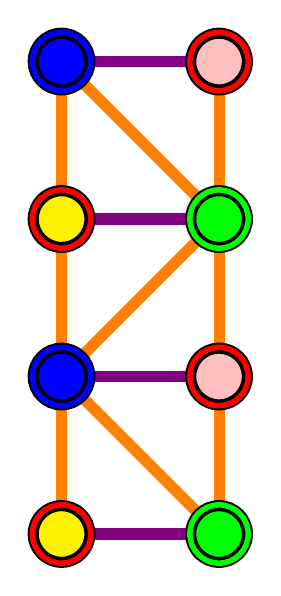
\begin{tikzpicture}
    \draw [violet, line width = 4] (0,0) -- (2,0);
    \draw [violet, line width = 4] (0,2) -- (2,2);
    \draw [violet, line width = 4] (0,4) -- (2,4);
    \draw [violet, line width = 4] (0,6) -- (2,6);

    \draw [orange, line width = 4] (0,0) -- (0,2);
    \draw [orange, line width = 4] (0,2) -- (0,4);
    \draw [orange, line width = 4] (0,4) -- (0,6);

    \draw [orange, line width = 4] (2,0) -- (2,2);
    \draw [orange, line width = 4] (2,2) -- (2,4);
    \draw [orange, line width = 4] (2,4) -- (2,6);

    \draw [orange, line width = 4] (2,0) -- (0,2);
    \draw [orange, line width = 4] (0,2) -- (2,4);
    \draw [orange, line width = 4] (2,4) -- (0,6);

    \path [draw = black, fill = yellow, line width = 4] (0,0) circle [radius = 0.36];
    \path [draw = black, fill = green,  line width = 4] (2,0) circle [radius = 0.36];
    \path [draw = black, fill = blue,   line width = 4] (0,2) circle [radius = 0.36];
    \path [draw = black, fill = pink,   line width = 4] (2,2) circle [radius = 0.36];
    \path [draw = black, fill = yellow, line width = 4] (0,4) circle [radius = 0.36];
    \path [draw = black, fill = green,  line width = 4] (2,4) circle [radius = 0.36];
    \path [draw = black, fill = blue,   line width = 4] (0,6) circle [radius = 0.36];
    \path [draw = black, fill = pink,   line width = 4] (2,6) circle [radius = 0.36];

    \path [draw = red,   line width = 2] (0,0) circle [radius = 0.37];
    \path [draw = green, line width = 2] (2,0) circle [radius = 0.37];
    \path [draw = blue,  line width = 2] (0,2) circle [radius = 0.37];
    \path [draw = red,   line width = 2] (2,2) circle [radius = 0.37];
    \path [draw = red,   line width = 2] (0,4) circle [radius = 0.37];
    \path [draw = green, line width = 2] (2,4) circle [radius = 0.37];
    \path [draw = blue,  line width = 2] (0,6) circle [radius = 0.37];
    \path [draw = red,   line width = 2] (2,6) circle [radius = 0.37];
\end{tikzpicture}
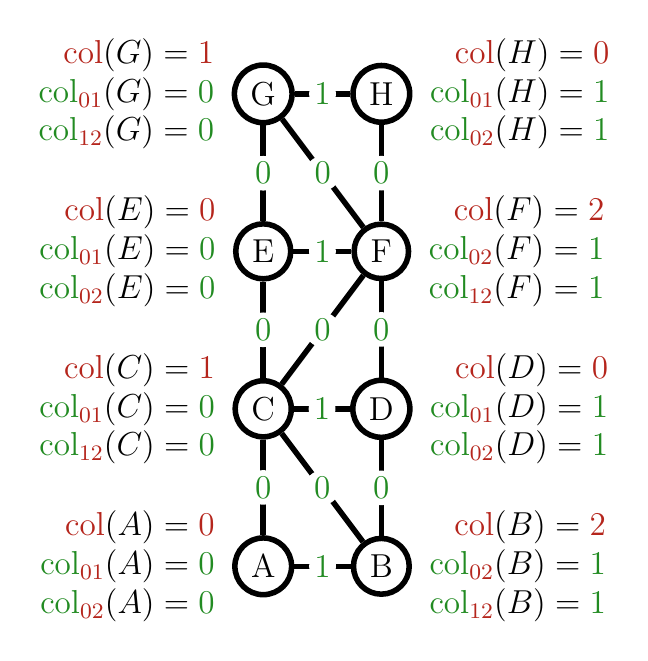
\begin{tikzpicture}[line width=2]
    \begin{scope}[every node/.append style={draw, circle, node font=\large, inner sep=3pt}]
	\node (A) at (0,  0) {A};
	\node (B) at (1.5,0) {B};
	\node (C) at (0,  2) {C};
	\node (D) at (1.5,2) {D};
	\node (E) at (0,  4) {E};
	\node (F) at (1.5,4) {F};
	\node (G) at (0,  6) {G};
	\node (H) at (1.5,6) {H};
    \end{scope}

    \begin{scope}[every node/.append style={fill=white, node font=\large\edgecolor, circle, inner sep=1pt}]
	\draw (A) -- node [inner sep = 0] {1} (B) (C) -- node [inner sep=0] {1} (D) (E) -- node [inner sep=0] {1} (F) (G) -- node [inner sep=0] {1} (H);
	\draw (A) -- node {0} (C) -- node {0} (E) -- node {0} (G);
	\draw (B) -- node {0} (D) -- node {0} (F) -- node {0} (H);
	\draw (B) -- node {0} (C) -- node {0} (F) -- node {0} (G);
    \end{scope}

    % Node colors
    \node [left=0.05 of A, anchor=east, align=right, node font=\large] {$\v\col(A)=\v0$\\$\e\col_{\v{01}}(A)=\e0$\\$\e\col_{\v{02}}(A)=\e0$};
    \node [left=0.05 of C, anchor=east, align=right, node font=\large] {$\v\col(C)=\v1$\\$\e\col_{\v{01}}(C)=\e0$\\$\e\col_{\v{12}}(C)=\e0$};
    \node [left=0.05 of E, anchor=east, align=right, node font=\large] {$\v\col(E)=\v0$\\$\e\col_{\v{01}}(E)=\e0$\\$\e\col_{\v{02}}(E)=\e0$};
    \node [left=0.05 of G, anchor=east, align=right, node font=\large] {$\v\col(G)=\v1$\\$\e\col_{\v{01}}(G)=\e0$\\$\e\col_{\v{12}}(G)=\e0$};

    \node [right=0.05 of B, anchor=west, align=right, node font=\large] {$\v\col(B)=\v2$\\$\e\col_{\v{02}}(B)=\e1$\\$\e\col_{\v{12}}(B)=\e1$};
    \node [right=0.05 of D, anchor=west, align=right, node font=\large] {$\v\col(D)=\v0$\\$\e\col_{\v{01}}(D)=\e1$\\$\e\col_{\v{02}}(D)=\e1$};
    \node [right=0.05 of F, anchor=west, align=right, node font=\large] {$\v\col(F)=\v2$\\$\e\col_{\v{02}}(F)=\e1$\\$\e\col_{\v{12}}(F)=\e1$};
    \node [right=0.05 of H, anchor=west, align=right, node font=\large] {$\v\col(H)=\v0$\\$\e\col_{\v{01}}(H)=\e1$\\$\e\col_{\v{02}}(H)=\e1$};
\end{tikzpicture}
\end{document}
